\documentclass[11pt]{article}
\usepackage{hyperref}
\usepackage{tabularx}
\usepackage{graphicx}
\usepackage{scalerel,stackengine}
\stackMath
\newcommand\reallywidehat[1]{%
\savestack{\tmpbox}{\stretchto{%
  \scaleto{%
    \scalerel*[\widthof{\ensuremath{#1}}]{\kern-.6pt\bigwedge\kern-.6pt}%
    {\rule[-\textheight/2]{1ex}{\textheight}}%WIDTH-LIMITED BIG WEDGE
  }{\textheight}% 
}{0.5ex}}%
\stackon[1pt]{#1}{\tmpbox}%
}
\parskip 1ex
\graphicspath{ {./images/}}
%%%%%%%%%%%%%%%%%%%%%%%%%%%%%%%%%%%%%%%%%
% Lachaise Assignment
% Structure Specification File
% Version 1.0 (26/6/2018)
%
% This template originates from:
% http://www.LaTeXTemplates.com
%
% Authors:
% Marion Lachaise & François Févotte
% Vel (vel@LaTeXTemplates.com)
%
% License:
% CC BY-NC-SA 3.0 (http://creativecommons.org/licenses/by-nc-sa/3.0/)
% 
%%%%%%%%%%%%%%%%%%%%%%%%%%%%%%%%%%%%%%%%%

%----------------------------------------------------------------------------------------
%	PACKAGES AND OTHER DOCUMENT CONFIGURATIONS
%----------------------------------------------------------------------------------------

\usepackage{amsmath,amsfonts,stmaryrd,amssymb} % Math packages

\usepackage{enumerate} % Custom item numbers for enumerations

\usepackage[ruled]{algorithm2e} % Algorithms

\usepackage[framemethod=tikz]{mdframed} % Allows defining custom boxed/framed environments

\usepackage{listings} % File listings, with syntax highlighting
\lstset{
	basicstyle=\ttfamily, % Typeset listings in monospace font
}

%----------------------------------------------------------------------------------------
%	DOCUMENT MARGINS
%----------------------------------------------------------------------------------------

\usepackage{geometry} % Required for adjusting page dimensions and margins

\geometry{
	paper=a4paper, % Paper size, change to letterpaper for US letter size
	top=2.5cm, % Top margin
	bottom=3cm, % Bottom margin
	left=2.5cm, % Left margin
	right=2.5cm, % Right margin
	headheight=14pt, % Header height
	footskip=1.5cm, % Space from the bottom margin to the baseline of the footer
	headsep=1.2cm, % Space from the top margin to the baseline of the header
	%showframe, % Uncomment to show how the type block is set on the page
}

%----------------------------------------------------------------------------------------
%	FONTS
%----------------------------------------------------------------------------------------

\usepackage[utf8]{inputenc} % Required for inputting international characters
\usepackage[T1]{fontenc} % Output font encoding for international characters

\usepackage{XCharter} % Use the XCharter fonts

%----------------------------------------------------------------------------------------
%	COMMAND LINE ENVIRONMENT
%----------------------------------------------------------------------------------------

% Usage:
% \begin{commandline}
%	\begin{verbatim}
%		$ ls
%		
%		Applications	Desktop	...
%	\end{verbatim}
% \end{commandline}

\mdfdefinestyle{commandline}{
	leftmargin=10pt,
	rightmargin=10pt,
	innerleftmargin=15pt,
	middlelinecolor=black!50!white,
	middlelinewidth=2pt,
	frametitlerule=false,
	backgroundcolor=black!5!white,
	frametitle={Command Line},
	frametitlefont={\normalfont\sffamily\color{white}\hspace{-1em}},
	frametitlebackgroundcolor=black!50!white,
	nobreak,
}

% Define a custom environment for command-line snapshots
\newenvironment{commandline}{
	\medskip
	\begin{mdframed}[style=commandline]
}{
	\end{mdframed}
	\medskip
}

%----------------------------------------------------------------------------------------
%	FILE CONTENTS ENVIRONMENT
%----------------------------------------------------------------------------------------

% Usage:
% \begin{file}[optional filename, defaults to "File"]
%	File contents, for example, with a listings environment
% \end{file}

\mdfdefinestyle{file}{
	innertopmargin=1.6\baselineskip,
	innerbottommargin=0.8\baselineskip,
	topline=false, bottomline=false,
	leftline=false, rightline=false,
	leftmargin=1cm,
	rightmargin=1cm,
	singleextra={%
		\draw[fill=black!10!white](P)++(0,-1.2em)rectangle(P-|O);
		\node[anchor=north west]
		at(P-|O){\ttfamily\mdfilename};
		%
		\def\l{3em}
		\draw(O-|P)++(-\l,0)--++(\l,\l)--(P)--(P-|O)--(O)--cycle;
		\draw(O-|P)++(-\l,0)--++(0,\l)--++(\l,0);
	},
	nobreak,
}

% Define a custom environment for file contents
\newenvironment{file}[1][File]{ % Set the default filename to "File"
	\medskip
	\newcommand{\mdfilename}{#1}
	\begin{mdframed}[style=file]
}{
	\end{mdframed}
	\medskip
}

%----------------------------------------------------------------------------------------
%	NUMBERED QUESTIONS ENVIRONMENT
%----------------------------------------------------------------------------------------

% Usage:
% \begin{question}[optional title]
%	Question contents
% \end{question}

\mdfdefinestyle{question}{
	innertopmargin=1.2\baselineskip,
	innerbottommargin=0.8\baselineskip,
	roundcorner=5pt,
	nobreak,
	singleextra={%
		\draw(P-|O)node[xshift=1em,anchor=west,fill=white,draw,rounded corners=5pt]{%
		Question \theQuestion\questionTitle};
	},
}

\newcounter{Question} % Stores the current question number that gets iterated with each new question

% Define a custom environment for numbered questions
\newenvironment{question}[1][\unskip]{
	\bigskip
	\stepcounter{Question}
	\newcommand{\questionTitle}{~#1}
	\begin{mdframed}[style=question]
}{
	\end{mdframed}
	\medskip
}

%----------------------------------------------------------------------------------------
%	WARNING TEXT ENVIRONMENT
%----------------------------------------------------------------------------------------

% Usage:
% \begin{warn}[optional title, defaults to "Warning:"]
%	Contents
% \end{warn}

\mdfdefinestyle{warning}{
	topline=false, bottomline=false,
	leftline=false, rightline=false,
	nobreak,
	singleextra={%
		\draw(P-|O)++(-0.5em,0)node(tmp1){};
		\draw(P-|O)++(0.5em,0)node(tmp2){};
		\fill[black,rotate around={45:(P-|O)}](tmp1)rectangle(tmp2);
		\node at(P-|O){\color{white}\scriptsize\bf !};
		\draw[very thick](P-|O)++(0,-1em)--(O);%--(O-|P);
	}
}

% Define a custom environment for warning text
\newenvironment{warn}[1][Warning:]{ % Set the default warning to "Warning:"
	\medskip
	\begin{mdframed}[style=warning]
		\noindent{\textbf{#1}}
}{
	\end{mdframed}
}

%----------------------------------------------------------------------------------------
%	INFORMATION ENVIRONMENT
%----------------------------------------------------------------------------------------

% Usage:
% \begin{info}[optional title, defaults to "Info:"]
% 	contents
% 	\end{info}

\mdfdefinestyle{info}{%
	topline=false, bottomline=false,
	leftline=false, rightline=false,
	nobreak,
	singleextra={%
		\fill[black](P-|O)circle[radius=0.4em];
		\node at(P-|O){\color{white}\scriptsize\bf i};
		\draw[very thick](P-|O)++(0,-0.8em)--(O);%--(O-|P);
	}
}

% Define a custom environment for information
\newenvironment{info}[1][Info:]{ % Set the default title to "Info:"
	\medskip
	\begin{mdframed}[style=info]
		\noindent{\textbf{#1}}
}{
	\end{mdframed}
}
 

\title{AMS 572 Fall 2020 Group 17 Project}

\author{
  Kai Li\thanks{Department of Applied Mathematics and Statistics, Stony Brook University, email: \href{mailto:Kai.Li@stonybrook.edu}{Kai.Li@stonybrook.edu}}\and
  Yunhan Qi\thanks{Department of Applied Mathematics and Statistics, Stony Brook University, email: \href{mailto:Yunhan.Qi@stonybrook.edu}{Yunhan.Qi@stonybrook.edu}}\and
  Tiange Zhang\thanks{Department of Applied Mathematics and Statistics, Stony Brook University, email: \href{mailto:Tiange.Zhang@stonybrook.edu}{Tiange.Zhang@stonybrook.edu}}
}

\date{Stony Brook University --- \today}

\begin{document}
\maketitle

\section{Introduction}
Statistics is the science of collecting and analyzing data to make conclusions and reach decisions \cite{bk:tamhane_dunlop}. This group project will analyze a data set from the SENIC Project \cite{ar:senic} using data analysis techniques learned in AMS 572 to identify patterns and draw inferences from the data. 

The data set follows the project guidelines because it contains 113 samples and 12 continuous, categorical variables. Moreover, the data set is legitimate since there are persuading reasons to present the methodology of the SENIC Project that lead to the data result, which shows the credibility of the data set \cite{ar:eickhoff}. Moreover, there is a detailed description in \cite{ar:eickhoff} discussing the sampling procedures and methodology used in the SENIC Project. Therefore, we are confident that the data set is reliable for doing data analysis.

The data set is stored as a Microsoft Excel Open XML Spreadsheet (XLSX) file created by Microsoft Excel. In this project, we will use the R language and environment to do statistical computing and graphics work. Before doing hypotheses testing of interests, we need to import the data set file into R, which requires installing a package called "readxl" so that R can load the data set:
\begin{file}[hospital.r]
\begin{lstlisting}[language = R]
install.packages("readxl")
library("readxl")
data <- read_excel("~/Desktop/hospital.xlsx")
\end{lstlisting}
\end{file}

\begin{info}\label{info}
The primary objective of the Study on the Efficacy of Nosocomial Infection Control (\textbf{SENIC} Project) was to determine whether infection surveillance and control programs have reduced the rates of nosocomial (hospital-acquired) infection in United States hospitals. This data set consists of a random sample of 113 hospitals selected from the original 338 hospitals surveyed. 

Each line of the data set has an identification number and provides information on 11 other variables for a single hospital. The data presented here are for the 1975-76 study period. The 12 variables are:
\end{info}
\begin{table}[h]
\begin{center}
\label{tab:table1}
\begin{tabularx}{\textwidth}{p{2.7cm}p{3.8cm}p{8.4cm}}
\hline
\textbf{Variable Number} & \textbf{Variable Name} & \textbf{Description} \\ 
\hline
1  & Identification number             & 1-113 \\
2  & Length of stay                    & Average length of stay of all patients in hospital (in days) \\
3  & Age                               & Average ages of patients (in years)\\
4  & Infection risk                    & Average estimated probability of acquiring infection in hospital (in percent) \\
5  & Routine culturing ratio           & Ratio of number of cultures performed to number of patients without signs or symptoms of hospital-acquired infection, times 100 \\
6  & Routine chest X-ray ratio         & Ratio of number of X-rays performed to number of patients without signs or symptoms of hospital-acquired infection, times 100 \\
7  & Number of beds                    & Average number of beds in hospital during study period \\
8  & Medical school affiliation        & 1=Yes, 2=No \\
9  & Region                            & Geographic region, where: 1=NE, 2=NC, 3=S, 4=W \\
10 & Average daily census              & Average number of patients in hospital per day during study period \\
11 & Number of nurses                  & Average number of full-time equivalent registered and licensed practical nurses during study period (number full time plus one half the number part time) \\
12 & Available facilities and services & Percent of 35 potential facilities and services that are provided by the hospital \\
\hline
\end{tabularx}
\end{center}
\end{table}

In the above script editor \textit{hospital.r}, we suppose a Mac user stores the excel data file named "hospital.xlsx" located at "Desktop". We can verify whether we import the correct data or not by typing the following in the command line:
\begin{commandline}
\begin{verbatim}
> dim(data)
[1] 113  12
\end{verbatim}
\end{commandline}
\textit{dim()} is a function in R that retrieves the dimension of the data. There are 113 rows and three columns, which match the number of samples and variables in the data set, as described in \hyperref[info]{info}. If we want to furtherly verify the variable names and their values in the file, we can do this by using the \textit{str()} function:
\begin{commandline}
\begin{verbatim}
> str(data)
tibble [113 x 12] (S3: tbl_df/tbl/data.frame)
 $ indentification number           : num [1:113] 1 2 3 4 5 6 7 8 9 ...
 $ length of stay                   : num [1:113] 7.13 8.82 8.34 8.95 ...
 $ age                              : num [1:113] 55.7 58.2 56.9 53.7 ...
 $ infection risk                   : num [1:113] 4.1 1.6 2.7 5.6 5.7 ...
 $ routine culturing ratio          : num [1:113] 9 3.8 8.1 18.9 34.5 ...
 $ routine chest X-ray ratio        : num [1:113] 39.6 51.7 74 122.8 ...
 $ number of beds                   : num [1:113] 279 80 107 147 180 ...
 $ medical school affiliation       : num [1:113] 2 2 2 2 2 2 2 1 2 2 ...
 $ region                           : num [1:113] 4 2 3 4 1 2 3 2 3 1 ...
 $ average daily census             : num [1:113] 207 51 82 53 134 ...
 $ number of nurses                 : num [1:113] 241 52 54 148 151 ...
 $ avaliable facilities and services: num [1:113] 60 40 20 40 40 40 ...
\end{verbatim}
\end{commandline}
In the above command, the \textit{str()} function displays the overall structure of the data, such as the dimension of the data set, variable names, and some of their values. Therefore, we can easily see that the data set is successfully imported into R. Then, we can proceed to do statistical analysis. 


\section{Hypotheses of Interests}
\subsection{Hypothesis Test on Mean}

\begin{question}
Refer to the data set from the SENIC Project. We want to know if the mean length of stay $\mu$ of all patients in the sample hospitals is different from 9 days. A two-sided hypothesis test on $\mu$ is appropriate to answer this question. Perform the hypothesis test at the 5\% level of significance using the following three ways:
\begin{enumerate}[(1)]
		\item Calculate the test statistic.
		\item Calculate the \textit{P}-value.
		\item Calculate a $95\%$ confidence interval for $\mu$.
\end{enumerate}
\end{question}\label{ques_1}

First, we formulate $\textit{H}_0$ and $\textit{H}_1$, and specify $\alpha$: $\textit{H}_0$: $\mu = 9$\, vs.\, $\textit{H}_1$: $\mu \neq 9$,\, $\alpha = 0.05$.

In this example, we will use the student's $t$-statistic to obtain a precise result. Before performing a $t$-test, we need to check if there exist observations larger than the 75th percentile plus 1.5 times of the interquartile range or less than the 25th percentile minus 1.5 times of the interquartile range, which are called outliers. Mathematically speaking, we want
\begin{align*}
\textrm{largest observation}&\leq \hat{\zeta}_{.75}+1.5\,\times\,\textrm{IQR},\\
\textrm{smallest observation}&\geq \hat{\zeta}_{.25}-1.5\,\times\,\textrm{IQR}.
\end{align*}
We will verify the conditions by drawing a boxplot of the variable \textit{length of stay}. If both conditions are satisfied, we may proceed to perform the statistical analysis. If not, then a technique learned in AMS 572 is to plot the data beyond whiskers individually.
\begin{commandline}
\begin{verbatim}
> box_vals <- boxplot(data$`length of stay`, ylab = "length of stay")$out
\end{verbatim}
\end{commandline}

\begin{figure}[h!]
\begin{center}\label{boxplot}
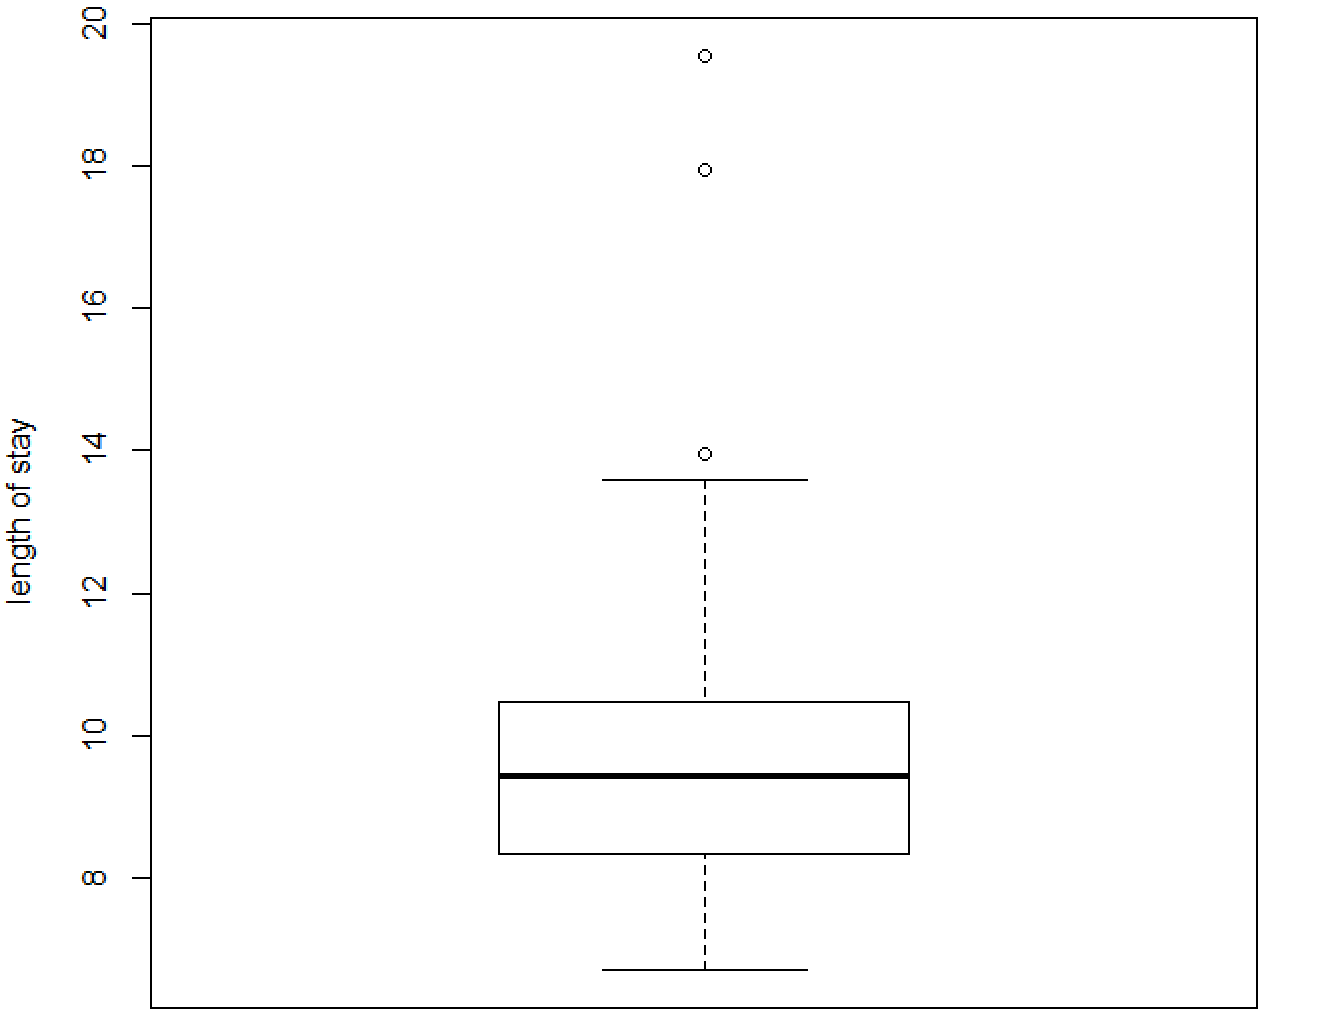
\includegraphics[scale=0.5]{boxplot}
\end{center}\caption{A boxplot of \textit{length of stay}.}
\end{figure}

\noindent The three outliers shown in \hyperref[boxplot]{Figure 1} violate our guidelines for the largest observation. Therefore, we drop the three observations in our data set to proceed with regression analysis and hypotheses testing. Since only a few observations drop compared to the sample size, we will not investigate the outliers in the project. The following shows the procedure to drop unwanted outliers:
\begin{file}[hospital.r]
\begin{lstlisting}[language = R]
outliers <- which(data$`length of stay` %in% box_vals)
data_new <- data[-outliers,]
\end{lstlisting}
\end{file}

Now, we are ready to do hypothesis testing. For the student's $t$-test, we need to know whether the data set follows a normal distribution or not
so that we can apply the $t$-test statistic. We can assess whether the normal distribution model is a proper fit or not both graphically and statistically. Graphically speaking, a quantile-quantile (Q-Q) plot is helpful in evaluation:

\begin{commandline}
\begin{verbatim}
> qqnorm(data_new$`length of stay`, ylab = "length of stay",
         pch = 1, frame = FALSE)
> qqline(data_new$`length of stay`, col = "red", lwd = 2)
\end{verbatim}
\end{commandline}

\begin{figure}[h!]\label{qqplot}
\begin{center}
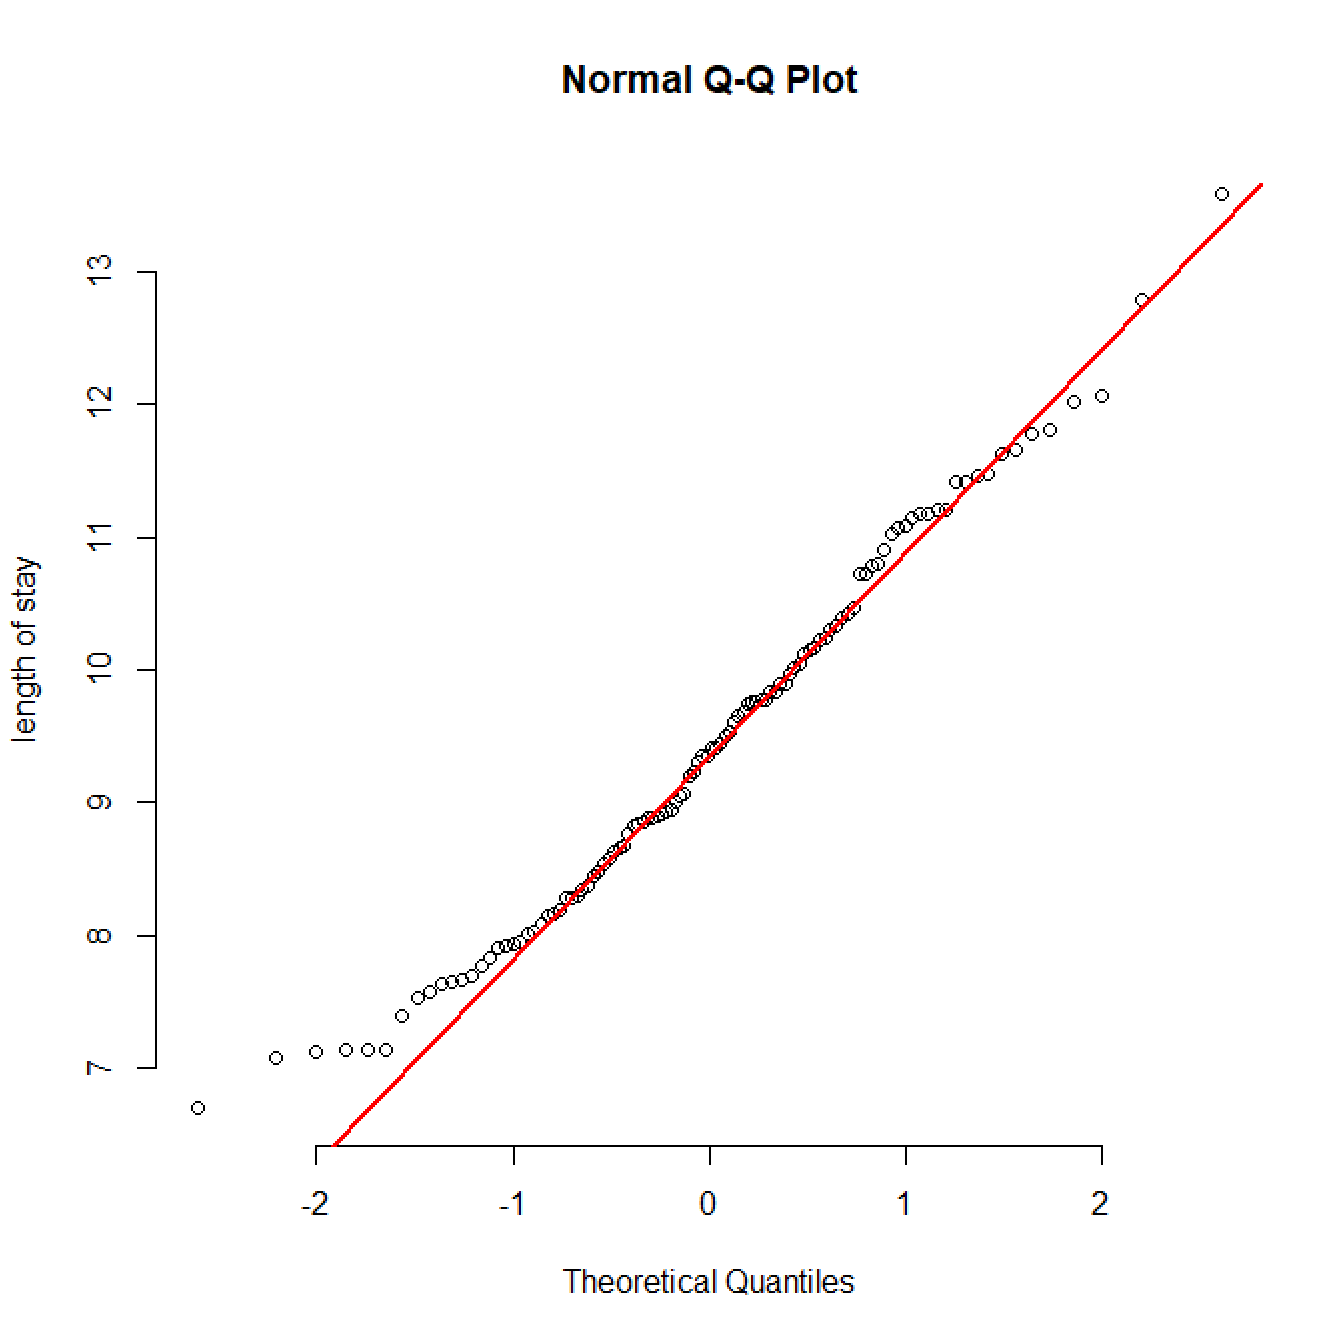
\includegraphics[scale=0.5]{qq}
\end{center}\caption{A Q-Q Plot of \textit{length of stay}.}
\end{figure}

\noindent Based on \hyperref[qqplot]{Figure 2}, most of the points follow the red straight normal line, indicating the normality assumption reasonable, graphically speaking.

We can also verify the normality assumption using the Shapiro-Wilk statistical test. Shapiro-Wilk test has the most power for different distributions and sample sizes than Kolmogorov-Smirnov, Lilliefors, and Anderson-Darling Tests \cite{ar:razali_yap}.
\begin{commandline}
\begin{verbatim}
> shapiro.test(data_new$`length of stay`)

        Shapiro-Wilk normality test

data:  data_new$`length of stay`
W = 0.98184, p-value = 0.1398
\end{verbatim}
\end{commandline}
At 5\% level of significance, because the $p\textrm{-value}=0.1398>0.05$, we fail to reject that the given data set does not follow a normal distribution. The conclusion matches the graphical result given in \hyperref[qqplot]{Figure 2}. Hence, we can assume the data is normal and proceed to do the $t$-test. \textit{t.test()} is the function in R that performs the $t$-test.

\begin{commandline}
\begin{verbatim}
> t.test(data_new$`length of stay`, mu = 9)

        One Sample t-test

data:  data_new$`length of stay`
t = 3.2824, df = 109, p-value = 0.001383
alternative hypothesis: true mean is not equal to 9
95 percent confidence interval:
 9.175800 9.711654
sample estimates:
mean of x 
 9.443727 
\end{verbatim}
\end{commandline}

Now, we are able to answer \hyperref[ques_1]{Question 1} given the above results:
\begin{enumerate}[(1)]    
    \item $t\textrm{-statistic}=3.2824$. Here $\alpha=0.05$, so $t_{\alpha/2,\, 109}=1.984$. Since $\lvert t \rvert=3.2824>1.984$, we reject $\textit{H}_0$ and conclude that the mean length of stay $\mu$ of all patients in hospital is different from $9$ days. 
    \item $p\textrm{-value}=0.001383$. This tells us that if the true length of stay mean is $\mu=9$ days, the probability of obtaining a sample mean that is different by 0.443737 days from the true mean is only 0.001383. Since this probability is less than $\alpha=0.05$, we reject $\textit{H}_0$.
    \item 95\% CI for $\mu$: $[9.175800,\, 9.711654]$. Since $\mu_{0}=9$ does not fall in this CI, we reject $\textit{H}_0$.
\end{enumerate}


\subsection{Hypothesis Test on Regression Coefficients with the Effect of Missing Values}
In this section, we will investigate the effect of missing values on data analysis for two scenarios: 

\begin{itemize}
\item Missing values are at completely random (Section \ref{sec:2.2.1}).
\item Missing values are non-ignorable (not random) (Section \ref{sec:2.2.2}).
\end{itemize}


\subsubsection{Missing Values at Completely Random (MCAR)}\label{sec:2.2.1}
Data can be regarded as MCAR if data are missing because of design issues, such as an equipment failure, technical problems, or samples lost in transit \cite{ar:kang}. In this project, we hypothesize the scenario by choosing 20\% of the data missing at completely random, as suggested in the project requirement. In other words, we need to randomly select our current data set so that we have 80\% of the data remaining:
\begin{file}[hospital.r]
\begin{lstlisting}[language = R] 
data_rand <- data_new[sample(nrow(data_new), 
                      ceiling(0.8*nrow(data_new))),]
\end{lstlisting}
\end{file}
We may wish to check if 20\% of the original data set is removed by looking at its dimension:

\begin{commandline}
\begin{verbatim}
> dim(data_rand)
[1] 88  12
\end{verbatim}
\end{commandline}
It turns out that indeed 20\% of data is dropped, ($88=0.8\times(113-3)$), where 113 is the total number of samples in the original data set, and 3 is the number of outliers dropped after concluding from \hyperref[boxplot]{Figure 1}. If we want to look at the structure of the modified data set in a more detailed sense, we can use the \textit{str()} function, similar to the commands used in the original data:
\begin{commandline}
\begin{verbatim}
> str(data_new)
tibble [88 x 12] (S3: tbl_df/tbl/data.frame)
 $ indentification number           : num [1:88] 4 108 86 85 61 5 82 ...
 $ length of stay                   : num [1:88] 8.95 8.02 9.05 8.09 ...
 $ age                              : num [1:88] 53.7 55 51.2 56.9 58 ...
 $ infection risk                   : num [1:88] 5.6 2.1 4.1 1.7 3.4 ...
 $ routine culturing ratio          : num [1:88] 18.9 3.8 20.5 7.6 8 ...
 $ routine chest X-ray ratio        : num [1:88] 122.8 46.5 79.8 56.9 ...
 $ number of beds                   : num [1:88] 147 91 195 92 119 ...
 $ medical school affiliation       : num [1:88] 2 2 2 2 2 2 2 2 2 1 ...
 $ region                           : num [1:88] 4 2 3 3 1 1 2 1 2 3 ...
 $ average daily census             : num [1:88] 53 44 127 61 67 134 ...
 $ number of nurses                 : num [1:88] 148 32 112 61 64 151 ...
 $ avaliable facilities and services: num [1:88] 40 22.9 45.7 45.7 ...
\end{verbatim}
\end{commandline}

Currently, the MCAR condition has been imposed. From the perspective of statistics, though power may decrease due to deficiency in the design, statistical analysis remains unbiased even if the data set is MCAR \cite{ar:kang}. Therefore, the estimated parameters are unbiased, though a portion of data lacks at completely random \cite{ar:kang}. As a result, we can do regression analysis like usual in this case. We begin by stating the second question.

\begin{question}
Refer to the modified data set which drops 20\% of the observations from the SENIC Project data set. Suppose that we are interested in the factors that influence whether a hospital is affiliated with a medical school or not. Particularly, we are interested in the effects of the average estimated probability of acquiring infection in a hospital, the hospital's geographic region and the average number of patients in the hospital per day during the study period to the medical school affiliation with the hospital. Fit a logit model to the modified data set to explain the effects between the variables, and perform hypotheses tests for both individual predictor variable effect and joint predictor variables effects on the response variable.
\end{question}

The response variable \textit{medical school affiliation} is binary, or sometimes called dummy. It means that the value takes either 1 or 0, meaning either affiliation exists or not, respectively. The predictor variables of interests are \textit{infection risk}, \textit{region}, and \textit{average daily census}. We will regard the variables \textit{infection risk} and \textit{average daily census} as continuous. The variable \textit{region} takes on the values 1, 2, 3, and 4, which represents four different geographical locations, NE, NC, S, and W.

Because \textit{region} is a categorical variable, we need to convert it to a factor before fitting the data to a regression. Then, because the data set uses 1 and 2 to represent "Yes" and "No", respectively, to denote the variable \textit{medical school affiliation}, we have to change all the 2's to 0's in \textit{medical school affiliation} so that it is binary.

\begin{file}[hospital.r]
\begin{lstlisting}[language = R]
data_rand$region <- factor(data_rand$region)
data_rand$`medical school affiliation` [data_rand$
          `medical school affiliation` %in% 2] <- 0
\end{lstlisting}
\end{file}
To check if the values are changed correctly, we can use the \textit{str()} function again:

\begin{commandline}
\begin{verbatim}
> str(data_rand)
tibble [88 x 12] (S3: tbl_df/tbl/data.frame)
 $ indentification number           : num [1:88] 4 108 86 85 61 5 82 ...
 $ length of stay                   : num [1:88] 8.95 8.02 9.05 8.09 ...
 $ age                              : num [1:88] 53.7 55 51.2 56.9 58 ...
 $ infection risk                   : num [1:88] 5.6 2.1 4.1 1.7 3.4 ...
 $ routine culturing ratio          : num [1:88] 18.9 3.8 20.5 7.6 8 ...
 $ routine chest X-ray ratio        : num [1:88] 122.8 46.5 79.8 56.9 ...
 $ number of beds                   : num [1:88] 147 91 195 92 119 ...
 $ medical school affiliation       : num [1:88] 0 0 0 0 0 0 0 0 0 1 ...
 $ region                           : Factor w/ 4 levels "1","2","3","4": 
 $ average daily census             : num [1:88] 53 44 127 61 67 134 ...
 $ number of nurses                 : num [1:88] 148 32 112 61 64 151 ...
 $ avaliable facilities and services: num [1:88] 40 22.9 45.7 45.7 ...
\end{verbatim}
\end{commandline}
The output indicates that all the 2's are switched to 0's while 1's are remaining the same in variable \textit{medical school affiliation}. The variable \textit{region} becomes a factor variable. 

Now, we are on track to estimate the parameters using a regression model. For this project, we are particularly interested in selecting a generalized linear model due to its unifying structure for analyzing linear and nonlinear regression models \cite{ar:m_p_c_m_b}. We also observe that our outcome of interest is a dummy variable, which can fit the logit or probit model. Because logistic regression is used in many medical fields \cite{ar:bagley_white_golomb}, we will conduct regression analysis and hypotheses testing using logit regression in this section.

Given the parameters of interests, the mathematical form of the linear relationship is 
\[
\begin{split}
\textrm{logit}\,\, p &= \ln\left(\frac{1}{1-p}\right)=\reallywidehat{\textrm{medical school affiliation}}\\
&=\beta_{0}+\beta_{1}\times\textrm{infection risk}+\beta_{2}\times\textrm{NC}+\beta_{3}\times\textrm{S}+\beta_{4}\times\textrm{W}+\beta_{5}\times\textrm{average daily census},
\end{split}
\]
where \textit{region2}, \textit{region3}, and \textit{region4} correspond
to geographical regions NC, S, and W, respectively. The following command 
uses the powerful \textit{glm()} function in R to fit the data using the logistic regression model:
\begin{file}[hospital.r]
\begin{lstlisting}[language = R] 
logit <- glm(`medical school affiliation` ~ 
             `infection risk` + region + 
             `average daily census`, data = data_rand, 
             family = binomial("logit"))
\end{lstlisting}
\end{file}

Now we have the regression results ready. By calling \textit{summary()} function in R, the command line window will pop out a simple summary of deviance residuals and each of the variable's coefficient estimate with a $p$-value:

\begin{commandline}
\begin{verbatim}
> summary(logit)

Call:
glm(formula = `medical school affiliation` ~ `infection risk` + 
    region + `average daily census`, family = binomial("logit"), 
    data = data_rand)

Deviance Residuals: 
     Min        1Q    Median        3Q       Max  
-1.67475  -0.31673  -0.21199  -0.06676   2.31649  

Coefficients:
                        Estimate Std. Error z value Pr(>|z|)    
(Intercept)            -4.760378   2.472857  -1.925 0.054223 .  
`infection risk`        0.007020   0.454154   0.015 0.987667    
region2                -0.713558   1.245734  -0.573 0.566779    
region3                -2.608358   1.475086  -1.768 0.077015 .  
region4                 0.498435   1.396239   0.357 0.721104    
`average daily census`  0.014698   0.004236   3.470 0.000521 ***
---
Signif. codes:  0 ‘***’ 0.001 ‘**’ 0.01 ‘*’ 0.05 ‘.’ 0.1 ‘ ’ 1

(Dispersion parameter for binomial family taken to be 1)

    Null deviance: 70.102  on 87  degrees of freedom
Residual deviance: 37.617  on 82  degrees of freedom
AIC: 49.617

Number of Fisher Scoring iterations: 7

\end{verbatim}
\end{commandline}

Thus, our logit regression model for the data set is
\begin{equation}
\begin{split}
\reallywidehat{\textrm{medical school affiliation}}=&-4.760+0.007\times\textrm{infection risk}-0.714\times\textrm{NC}-2.608\times\textrm{S}\\
&+0.498\times\textrm{W}+0.015\times\textrm{average daily census}
\end{split}
\end{equation}

The $p$-value of the individual restriction hypothesis testing is shown in the command output. The hypothesis can be written mathematically as
\[
\textit{H}_0:\,\beta_{i}=0\quad\textrm{vs.}\quad\textit{H}_1:\,\beta_{i}\neq0 \quad\textrm{for}\,\, i\in(1, 2, 3, 4, 5), \quad \alpha=0.05.
\]
Since the $p$-value of \textit{average daily census} is less than 5\%, the null hypothesis $\textit{H}_0:\,\beta_{5}=0$ can be rejected at 5\% significance level. For the intercept, \textit{infection risk}, and the three terms for \textit{region}, the coefficients are not statistically significant. Thus, we fail to reject the null hypotheses for those coefficients. That is, \textit{infection risk} and the three terms for \textit{region} do not have statistically significant effects on \textit{medical school affiliation}, and therefore indicating that the predictor variables are not useful predictors. Thus, \textit{infection risk} and \textit{region} can be dropped from the logit model and a simpler model can be formed with the remaining variable \cite{bk:tamhane_dunlop}.

We can use the \textit{confint()} function to obtain confidence intervals for the coefficient estimates. The CI's for each coefficient in the logit model can also assess the effect of each variable on the response variable, as shown in the following command \cite{bk:tamhane_dunlop}.

\begin{warn}[Notice:]
There are two functions that can produce an output of confidence intervals for the coefficients. One is \textit{confint()}, used in our case, to calculate confidence intervals by the profile likelihood method. The other one is \textit{confint.default()}, which calculates confidence intervals using standard errors.
\end{warn}

\begin{commandline}
\begin{verbatim}
> confint(logit)
Waiting for profiling to be done...
                               2.5 %      97.5 %
(Intercept)            -10.296161605 -0.38420774
`infection risk`        -0.922930674  0.89560526
region2                 -3.407397792  1.69459628
region3                 -5.945645358  0.06938331
region4                 -2.644778028  3.22431363
`average daily census`   0.007910323  0.02509251
\end{verbatim}
\end{commandline}
The confidence intervals generated using the profile likelihood method provide a slightly different result than the above single restriction hypothesis testing. In particular, the confidence interval for the intercept shows that we reject the null hypothesis that the intercept equals 0, which is the opposite conclusion obtained in the regression result. The conclusions for \textit{region} and \textit{average daily census} stay the same. Hence, we can conclude that variable \textit{average daily census} has statistically significant effect on \textit{medical school affiliation}, and thus a simplified model can be refitted with \textit{average daily census}.

Last but not least, we are interested in testing an overall effect of all variables \textit{infection risk}, \textit{region}, and \textit{average daily census}.  To see if the joint effect of the variables is statistically significant, we can use the \textit{wald.test()} function. The function is stored in the \textit{aod} library, and therefore we need to install the package \textit{aod}. To perform a joint hypothesis test on all coefficients of the variables, we can write the hypothesis mathematically, with a specified $\alpha$, as
\[
\textit{H}_0:\,\beta_{1}=\beta_{2}=\dots=\beta_{5}=0\quad\textrm{vs.}\quad\textit{H}_1:\,\textrm{at least one equality not true}, \quad \alpha=0.05.
\]

\begin{commandline}
\begin{verbatim}
> install.packages("aod")
> library(aod) 
> wald.test(b = coef(logit), Sigma = vcov(logit), Terms = 2:6)
Wald test:
----------

Chi-squared test:
X2 = 14.1, df = 5, P(> X2) = 0.015
\end{verbatim}
\end{commandline}
\textit{Terms}, as a paramter of \textit{wald.test()}, specifies which terms in the model are to be tested. $\beta_{0}$ corresponds to the intercept, the first term, and up to $\beta_{5}$ corresponds to the \textit{average daily census}, the sixth term. In this case, since we want to impose restrictions on regression coefficients for all variables, \textit{Terms} is from 2 to 6, excluding the first intercept term. 

The $p$-value of the chi-squared test is less than 0.05, and hence the joint null hypothesis that all the coefficients of the variables are 0 can be rejected at 5\% significance level. That is, we reject that none of the predictor variables are related to the response, and in favor of that at least one of the predictors is related to the response.

\subsubsection{Missing Values not at Random (MNAR)}\label{sec:2.2.2}
Some methods can handle missing values. However, the best practice is to prevent the problem by designing a well-planning experiment and collecting information carefully \cite{ar:desarbo_green_carroll, ar:w_l_o_t}. In the data set of the SENIC Project, nonresponse bias may occur in the following two scenarios during the sample selection process \cite{ar:senic2}:
\begin{itemize}
\item Noncoverage of the target population by the sampling frame\\\\
The SENIC Project study concerns both the sampling of hospitals and patients. The target population of hospitals, known as "the SENIC Universe", cannot be owned by federal or state; their locations have to be in one of the 48 states in the United States; they are short-term general medical and surgical hospitals that have at least 50 beds. The target population of patients has to be at least 18 years old, except for specific people with low risk of infection \cite{ar:senic2}. Hence, the non-ignorable missing values can be from any source mentioned above. Significantly, the sample considers both the population of hospitals and patients, which increases chances of nonresponse bias. 
\\
\item Replacement of initially participated hospitals but excluded from the sample subsequently due to different reasons\\\\
In this case, the SENIC sampling process article articulates six situations which resulted in the replacement: not being a member of the SENIC Universe as of 1976; participated in pilot studies; hospital closed after participating in the survey; non-participants; hospital records were deficient; and hospital implemented Infection Surveillance and Control Programs before 1969 \cite{ar:senic2}. Therefore, though hospitals may be targeted in the sample population, the missing values can be due to the later hospital replacement. Thus, nonresponse bias may occur not only in the sampling process, but also in the replacement process.\\
\end{itemize}

If there are missing values that are not at random, it is not simple to perfectly deal with the problem. One way to model the missing data is to use a more complex model, incorporated by the original model, to estimate the effect of the missing values unbiasedly \cite{ar:kang}. In particular, modeling and hypotheses testing on the replaced hospitals becomes a useful technique in clinical studies \cite{ar:senic2}. In response to patients' nonresponse bias, several differences between Preliminary Screening Questionnaire respondents and nonrespondents are compared to investigate the effect of missing values, to reduce the impact of nonresponse bias to the study \cite{ar:senic2}.


\bibliographystyle{abbrv}
\bibliography{refs}

\end{document}
